\centering
\begin{subfigure}{.5\textwidth}
  \centering
  %\begin{tikzpicture}
\begin{axis}[
	x tick label style={ /pgf/number format/1000 sep=},
	width=\cmpW, height=\cmpH,
	ylabel=Evaluations,
	ymode=log,
	grid = both,
	grid style={line width=.1pt, draw=gray!10},
	major grid style={line width=.2pt,draw=gray!50},
	%xlabel=Number of items (n),
	enlargelimits=0.15,
	legend style={at={(\legX,\legY)},
		anchor=north,legend columns=-1},
	ybar=2.6pt,% configures `bar shift'
	bar width=9pt,
	point meta=y *10^-7, % the displayed number
	cycle list = {black!80,black!30}
]

\addplot+[fill, text=black]
  coordinates {
    ( 40,3703070)
    ( 60,103534833)
    ( 80,700026931)
    (100,5542292786)
    (120,4935519921)
  };

\addplot+[fill, text=black]
  coordinates {
    ( 40,291655)
    ( 60,1182225)
    ( 80,5434379)
    (100,27996835)
    (120,31578018)
  };

\legend {AVL-tree,\dtree{2}}
\end{axis}
\end{tikzpicture}
  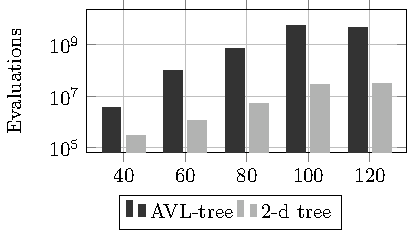
\includegraphics[scale=0.6]{tab/cmp/2dimA}
  \caption{Type A}
  \label{fig:sub1}
\end{subfigure}%
\begin{subfigure}{.5\textwidth}
  \centering
  %
\begin{tikzpicture}
\begin{axis}[
	x tick label style={ /pgf/number format/1000 sep=},
	width=\cmpW, height=\cmpH,
	ylabel=Avaliações,
	ymin=100000,
	ymax=100000000000,
	ymode=log,
	grid = both,
	grid style={line width=.1pt, draw=gray!10},
	major grid style={line width=.2pt,draw=gray!50},
	%xlabel=Number of items (n),
	enlargelimits=0.15,
	legend style={at={(\legX,\legY)},
		anchor=north,legend columns=-1},
	ybar=2pt,% configures `bar shift'
	bar width=8pt,
	xtick={100,200,300,400,500},
	xticklabels={100,200,300,400,500},
	point meta=y *10^-7, % the displayed number
	cycle list = {black!80,black!30}
]

\addplot+[fill, text=black]
  coordinates {
    (100,562886)
    (200,27327963)
    (300,349249789)
    (400,17406619609)
    (500,12137619611)
  };

\addplot+[fill, text=black]
  coordinates {
    (100,330881)
    (200,5329798)
    (300,396002213)
    (400,148865700)
    (500,318904809)
  };

\legend {AVL-tree,\dtree{2}}
\end{axis}
\end{tikzpicture}

  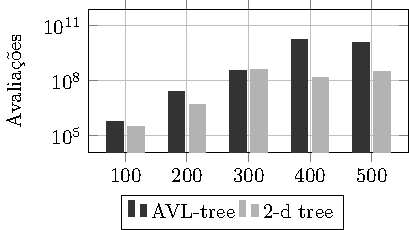
\includegraphics[scale=0.6]{tab/cmp/2dimB}
  \caption{Type B}
  \label{fig:sub2}
\end{subfigure}
\begin{subfigure}{.5\textwidth}
  \centering
  %
\begin{tikzpicture}
\begin{axis}[
	x tick label style={ /pgf/number format/1000 sep=},
	width=\cmpW, height=\cmpH,
	ylabel=Avaliações,
	ymin=100000,
	ymax=100000000000,
	ymode=log,
	grid = both,
	grid style={line width=.1pt, draw=gray!10},
	major grid style={line width=.2pt,draw=gray!50},
	%xlabel=Number of items (n),
	enlargelimits=0.15,
	legend style={at={(\legX,\legY)},
		anchor=north,legend columns=-1},
	ybar=2pt,% configures `bar shift'
	bar width=9pt,
	point meta=y *10^-7, % the displayed number
	cycle list = {black!80,black!30}
]

\addplot+[fill, text=black]
  coordinates {
    ( 20,191729)
    ( 40,18662815)
    ( 60,670819408)
    ( 80,4616460680)
    (100,73868244070)
  };

\addplot+[fill, text=black]
  coordinates {
    ( 20,32950)
    ( 40,926315)
    ( 60,5542258)
    ( 80,23285877)
    (100,80371740)
  };

\legend {AVL-tree,\dtree{2}}
\end{axis}
\end{tikzpicture}

  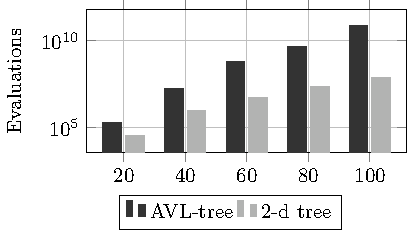
\includegraphics[scale=0.6]{tab/cmp/2dimC}
  \caption{Type C}
  \label{fig:sub3}
\end{subfigure}%
\begin{subfigure}{.5\textwidth}
  \centering
  %
\begin{tikzpicture}
\begin{axis}[
	x tick label style={ /pgf/number format/1000 sep=},
	width=\cmpW, height=\cmpH,
	ylabel=Avaliações,
	ymin=100000,
	ymax=100000000000,
	ymode=log,
	grid = both,
	grid style={line width=1.3pt, draw=gray!00},
	major grid style={line width=.2pt,draw=gray!50},
	%xlabel=Number of items (n),
	enlargelimits=0.15,
	legend style={at={(\legX,\legY)},
		anchor=north,legend columns=-1},
	ybar=2pt,% configures `bar shift'
	xmin=18,
	xmax=52,
	bar width=9pt,
	point meta=y *10^-7, % the displayed number
	cycle list = {black!80,black!30}
]

\addplot+[fill, text=black]
  coordinates {
    ( 20,2831448)
    ( 30,489772231)
    ( 40,9316773179)
    ( 50,19581372744)
  };

\addplot+[fill, text=black]
  coordinates {
    ( 20,173245)
    ( 30,3317384)
    ( 40,14262798)
    ( 50,57959241)
  };

\legend {AVL-tree,\dtree{2}}
\end{axis}
\end{tikzpicture}

  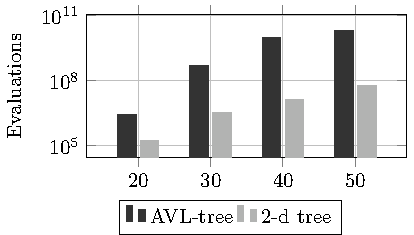
\includegraphics[scale=0.6]{tab/cmp/2dimD}
  \caption{Type D}
  \label{fig:sub4}
\end{subfigure}
